%\documentclass{article}

%\usepackage[utf8]{inputenc}
\usepackage{placeins}
\usepackage{graphicx}
\usepackage[ruled,vlined,linesnumbered]{algorithm2e}
\usepackage{listings}
\usepackage{amsthm}
\usepackage{amsmath}
\usepackage{caption}
\usepackage{epigraph}

\captionsetup[figure]{font=scriptsize}

\newtheorem{definition}{Definição}[section]
\theoremstyle{remark}
\newtheorem*{remark}{Observações}
\theoremstyle{theorem}
\newtheorem{theorem}{Teorema}[section]

\setlength{\parskip}{.5em}

\renewcommand\refname{Leituras adicionais}
\renewcommand\figurename{Figura}
\renewcommand{\lstlistingname}{Código}

\newcommand{\eclipse}{$ECL^iPS^e$}
\newcommand{\definicao}[1]{\textbf{#1}\marginpar{\small \textbf{#1}}}

\lstdefinestyle{prosty}{
  language=Prolog,
  basicstyle=\small
}




%\begin{document}
\section{Modelo Computacional de Programas Lógicos}

Considere o seguinte código:

\begin{listing}
  \inputminted{prolog}{../Exemplos/Cap1/prog1_circuito.pl}\label{lst:circuit}
  \caption{Circuito}
\end{listing}

A leitora pode se perguntar qual o resultado do seguinte goal:

\codigo{porta\_and(Entrada1, Entrada2, Saida)?}

Ela também pode se perguntar ``Será que, dado um programa qualquer e
um goal qualquer dá para ``calcular'' o resultado do goal?''.

% Note que, como o goal consiste contém variáveis (lembre-se que o que for capitalizado em programas lógicos denota uma variável), um resultado não é só \textit{sucesso} ou \textit{falha}, mas
% também, possivelmente, uma substituição para valores das variáveis (isto é, valores para as variáveis tal que o goal tenha sucesso).

Se houvesse muitos programas com goals de resultados incalculáveis,
programação lógica não seria tão útil e dificilmente teria sido feito
um material como este (mais difícil ainda é o material ter sido feito
e a leitora estar lendo), então esse não deve ser o caso, alguém
poderia dizer.

Se o goal estiver expresso no programa apenas como um fato base,
prová-lo é fácil: só precisamos checar se algum dos fatos é igual ao
goal. No caso mais geral, entretanto, se o goal conter alguma variável
ou só puder ser provado através de alguma regra, a situação pode ficar
mais complicada.

Se o goal contiver variáveis, para prová-lo precisamos encontrar uma
substituição para cada uma delas de forma que cada um dos termos do
goal seja logicamente consistente com o programa. Aqui o que queremos
dizer com ``substituição'' é que em todo lugar em que a variável
aparecer, ela é substituída por um outro termo (em outras palavras,
uma substituição $S$ é um conjunto, possivelmente vazio, de
atribuições de valores a variáveis).  Uma forma de pensar sobre isso é
que, antes da substituição, a variável ``tem uma vida só sua'', sendo
irrestrita, e que, depois, sua vida é, na verdade, ``a vida de
outro'', ou seja, é, em algum sentido, restrita. Mais precisamente,
temos:\\

% ' '*\\marginpar{\\textbf{*}} / \definicao{*}

\begin{definition} Dado um termo {\it p($a_1$, ..., $a_n$)}, onde os
$a_j$, para $j \in J$, $J$ algum conjunto indexador, são variáveis, uma
\definicao{substituição} é um conjunto $\iota$ de \definicao{unificações},
escritas como $a_i = k_j$, onde $k_j$ é uma variável ou um termo
atômico e ``='' indica que $a_i$ é idêntica a $k_j$ e dizemos que
$a_i$ é unificado com $k_j$.  Uma substituição $\iota$ sobre um programa P
é escrita P$\iota$.
\end{definition}

\begin{remark} \hfill
  \begin{enumerate}
  \item Ao realizar uma substituição $\iota$ sobre um programa P, o
    resultado é ou programa P$\iota$, sobre o qual podemos, em particular,
    fazer outras substituições;
  \item A relação ``$A = B$'' deve ser entendida como usado em álgebra
    (isto é, como denotando uma relação simétrica de igualdade entre
    $A$ e $B$) e não como geralmente usado em programação, como um
    operador de atribuição assimétrico (em que $A = b$ não é o mesmo
    que $b = A$);
  \item O símbolo ``='' expressa a relação de dois termos serem
    idênticos;
  \item Essa relação é transitiva: se A, B e C são variáveis
    e se \codigo{A = B} e \codigo{B = C}, então \codigo{A = C} (se A é
    idêntico a B e B é idêntico a C, então A é idêntico a C);
  \item Pelo item (2), não podemos fazer\footnote{Na verdade,
      podemos. Mas é como se não pudéssemos. Isso vai ficar mais claro
      quando lidarmos com \technical{backtracking}.} \codigo{A = 1} e,
    logo em seguida, \codigo{A = 2}: isso resulta em falha, por
    inconsistência. 
  \end{enumerate}
\end{remark}

Se temos que existe alguma substituição $\iota$ (possivelmente vazia) para
que $p(a_1, ..., a_n) = q(b_1, ..., b_n)$, dizemos que $p(a_1, ...,
a_n)$ é unificável com $q(b_1, ..., b_n)$. ``='' é o
\definicao{símbolo de unificação}\footnote{Veremos depois mais
predicados do tipo ``a op b'', onde op é o operador (no caso, op é
=/2). Predicados desse tipo são chamados de infixos. Todo predicado
infixo também pode ser usado no formato prefixo (como =(a, b) ) e
predicados infixos também podem ser definidos pelo programador, como
já mencionado anteriormente.}\footnote{ Rigorosamente, ``predicados''
são diferentes de ``funtores'', mas neste texto adotaremos a convenção
usual de nos referir a um ``funtor'' como ``predicado'' quando
quisermos enfatizar seu caráter procedural. }.

Convém notar aqui que, em Prolog, funtores são \enphasis{cidadãos de
primeira classe}, o que significa que compartilham o direito e
privilégio de ser nomeado por uma variável (isto é, uma variável pode
receber qualquer funtor n-ário, não só átomos).

Normalmente, quando lidando com outros tipos de linguagens, também
seria dito que:

\begin{enumerate}
\item Cidadãos de primeira classe podem ser retornados por funções e
passados como argumentos a elas e
\item Que podem ser incorporados em estruturas de dados.
\end{enumerate}

Como em programação lógica, a princípio, não fazemos uso de
funções\footnote{Em programação lógica pura não há funções no sentido
usual, mas nas encarnações concretas de programação lógica, elas
costumam aparecer de um jeito ou de outro.}, não podemos fazer a
afirmação 1, mas, na prática, o que dizemos é equivalente.  Isso
porque, apesar de um funtor \funtor{f/n} não retornar um valor
propriamente dito, se queremos um ``valor de retorno'', sempre podemos
fazer um \funtor{f/n+1}, cujo último argumento (ou qualquer outro, mas
costumamos optar pelo último pela conveniência de fazer apenas uma
escolha) seria o valor de retorno (como já foi visto no funtor
\funtor{length/2}, por exemplo) e o termo nessa última posição, se for
uma variável, pode ser unificado com um funtor. Quanto à afirmação 2,
podemos dizer somente que os funtores são o tijolo e cimento das
estruturas de dados em programação lógica.

Voltando ao tema das substituições, todas elas são iguais, mas algumas
são mais iguais que outras. Em particular, dado um programa P e
substituições $\iota$ e $\nu$, se existe alguma substituição $\eta$
tal que $(P\iota)\eta = P \nu$, dizemos que $\iota$ é uma substituição
mais geral do que $\nu$. A substituição mais geral é de especial
importância, porque podemos expressar outras substituições em função
dela.

Agora podemos expressar nosso objetivo de provar o goal a partir do
programa como o de achar uma substituição tal que cada termo do goal
seja unificável com alguma cláusula do programa. Mais precisamente, um
goal é provado a partir do programa se é possível unificar cada termo
do goal com alguma cláusula do programa de forma a preservar a
consistência das cláusulas. O processo pelo qual esse objetivo é
realizado é chamado \definicao{processo de resolução}.

Unificação exerce um papel fundamental na programação lógica. Na
prática, ele resume processos de atribuição de valores, gerenciamento
de memória, invocação de funções e passagem de valores, entre
outros. O primeiro estudo formal sobre unificação é devido a John
A. Robinson \cite{robinson}, que depois de montar um algoritmo de
unificação, gerou o primeiro de que temos conhecimento.

O algoritmo dele é um tanto ineficiente e só foi citado por
considerações históricas. Usaremos um outro no lugar. Antes, vale
lembrar que um programa lógico é um conjunto de regras que recebe um
goal (ou uma busca) e retorna \enphasis{sucesso} (ou, sim, ou
verdadeiro, dependendo da preferência pessoal) se a busca tem sucesso
ou \enphasis{falha} (ou, não, ou falso...) se não.

Como discutido acima, para provar um goal a partir de um programa é
suficiente que tenhamos um algoritmo de unificação. Esse algoritmo
recebe uma equação do tipo $T_1 = T_2$, e devolve uma substituição
mais geral\footnote{É importante que seja a mais geral, para não
perdermos possíveis soluções} para as variáveis presentes caso tal
substituição exista, ou falha, caso contrário. O algoritmo que
utilizaremos faz uso de uma pilha para armazenar as sub-equações a
serem resolvidas e de um espaço $\Gamma$ para armazenar a
substituições:

\begin{itemize}
\item[(a)] Faça o \technical{push}\footnote{Os \technical{push} e
    \technical{pop} devem ser entendidos como realizadas em uma pilha:
    \technical{push} põe um elemento na pilha, \technical{pop}
    retira.} da equação na pilha;
\item[(b)] Se a pilha estiver vazia, devolva sucesso. Se não, faça o
  \technical{pop} de um elemento (uma equação) $T_1 = T_2$ da
  pilha. Realize uma das ações a seguir, segundo a equação retirada:
  \begin{enumerate}
  \item Se $T_1$ e $T_2$ forem termos unários idênticos, nada precisa
    ser feito;
  \item Se $T_1$ é uma variável e $T_2$ um termo não contendo $T_1$,
    realize uma busca na pilha pelas ocorrências de $T_1$ e troque
    $T_1$ por $T_2$ (o mesmo é feito em $\Gamma$);
  \item Se $T_2$ for uma variável e $T_1$ for um termo não contendo
    $T_2$, a ação tomada é análoga ao do passo anterior;
  \item Se $T_1$ e $T_2$ forem termos compostos de mesmo funtor
    principal e aridade, $f(a_1, ..., a_n)$ e $p(b_1, ..., b_n)$,
    adicione as equações $a_i = b_i$ na pilha;
  \item Em outro caso, devolva falha.
  \end{enumerate}
\item[(c)] Retorne ao passo (b).
\end{itemize}


% % \begin{enumerate}
% % \item $f(k_1, ..., k_m) = p_i(t_1, ..., t_n)$, onde $m = n$, $f =
% p_i$: buscue as ocorrências troque as variáveis $t_l$ por $s_l$;
% % \item $f(k_1, ..., k_m) = p_i(t_1, ..., t_n)$, onde $f \neq p_i$:
% delete essa equação e pare, retorne com falha;
% % \item $x = x$: delete a equação;
% % \item $x = y$, onde $x$ é uma variável, mas $y$ não: troque $x$ por
% $y$ em todas as proposições consideradas;
% % \item $x = y$, onde $x$ é variável de $y$ (isto é, $y$ é algo como
% $y(a_1, ..., x, ..., a_n))$: pare e retorne com falha.
% % \end{enumerate}
% % \item[(c)] Se existe mais algum $p_i$ a ser escolhido, volte ao item
% (a), se não retorne com sucesso.
% % \end{itemize}

Intuitivamente, esse algoritmo tenta provar a equação de forma
construtiva: isto é, tenta construir uma solução por meio de
substituições e, se não chegar a uma contradição, termina com sucesso,
``devolvendo'' (não no sentido de uma função que devolve um valor, mas
no de ``mostrar'' ao usuário do programa) a substituição realizada.

Para provar um goal G, escolhemos não-deterministicamente\footnote{No
geral, podem existir várias escolhas possíveis e pode ser que, por
algumas sequências de escolhas de cláusulas, nunca cheguemos a uma
prova do goal, apesar de ele ser deduzível a partir de outras escolhas
de cláusulas. Quando dizemos que a escolha é não-determinística,
queremos dizer que, se existem mais de um conjuntos de escolhas que
provam o goal, um desses conjuntos é escolhido (a escolha é feita
entre as cláusulas que podem provar o goal, o que significa que, se
ele é provável, ele é provado). Na prática, isso pode ser implementado
apenas aproximadamente.  Ainda assim, é uma abstração importante e
leva a aplicações interessantes, na assim chamada,
\enphasis{programação não-determinística}. Em outros contextos, também
podemos usar esse mesmo termo para nos referir a situações nas quais o
programa tem, a princípio, mais de uma ``escolha'' (se não há
``escolhas'', dizemos que o contexto é determinístico).}  a cabeça de
uma cláusula T do programa, construímos uma equação do tipo \codigo{G
= T} e aplicamos o algoritmo acima. Caso ele devolva sucesso, fazemos
o mesmo com cada termo do corpo da cláusula. Caso devolva falha,
seleciona-se outra cláusula e é realizado o mesmo processo, até que
não haja mais cláusulas a serem selecionadas, quando o goal retorna
falha.

O passo 2.b do algoritmo merece uma explicação um pouco mais
detalhada. Ele diz implicitamente que x não é unificável com algum
\codigo{y(a\_1, ...,x, ...a\_n)}, isto é, com algum funtor que tome x
como argumento. Pode parecer estranho a princípio, mas a estranheza
some se se lembrar que funtor não é função: um funtor representa uma
estrutura primariamente simbólica. Sem essa condição, se \codigo{X =
y(a\_1, ..., X, ..., a\_n)}, então \codigo{X = y(a\_1, ...,y(a\_1,
..., x, ..., a\_n), ..., a\_n) = y(a\_1, ..., y(a\_1, ...,y(a\_1,
...,y(a\_1, ...,x, ..., a\_n), ..., a\_n) , ..., a\_n) , ..., a\_n)}
em um ciclo sem fim. Com um processo desses, não dá para provar um
goal e, portanto, é devolvida falha.

Para entender melhor, tome o exemplo do código \ref{lst:circuit}, no
início deste Capítulo, e suponha que àquele código é submetido o goal
\codigo{resistor(energia, n1)?} O algoritmo é aplicado como se segue:

\begin{enumerate}
\item Tentaremos a unificação do goal com a cláusula na primeira linha
do programa: a equação \codigo{resistor(energia, n1) =
resistor(energia, n1)} é posta na pilha;
\item Uma equação é retirada da pilha: a equação
\codigo{resistor(energia, n1) = resistor(energia, n1)};
\item A equação é formada por dois funtores termos compostos de mesmo
funtor principal e mesma aridade: as equações \codigo{energia =
energia} e \codigo{n1 = n1} são postas na pilha;
\item É retirada uma equação da pilha: a equação \codigo{energia =
energia}. Como os dois lados da equação são idênticos, não há mais o
que fazer;
\item É retirada outra equação da pilha: a equação \codigo{n1 =
n1}. Como os dois lados da equação são idênticos, não há mais o que
fazer;
\item A pilha está vazia: o programa devolve sucesso, com a
substituição $\Gamma = \{\}$ (substituição vazia).
\end{enumerate}

% TODO colocar mais exemplos

\subsection{Programas ``gera-e-testa''}

Programação não determinística não serve apenas para o desenvolvimento
da teoria de computação de programas lógicos, também serve como uma
abstração útil para a criação de programas interessantes.

Imagine que você se encontra em uma situação problemática e gostaria
de resolver o problema. Um procedimento possível é gerar uma provável
solução e, então, testar se ela de fato resolve o problema. Se formos
traduzir isso para programação lógica, teríamos algo como:

\begin{listing}
  \inputminted{prolog}{../Exemplos/Cap1/prog2_encontra.pl}
  \caption{Encontra}
\end{listing}

Para algum \enphasis{gera} e algum \enphasis{testa}. A hipótese de
não-determinísmo está na esperança de que será gerada uma solução que
passa no teste, o que não é, a princípio, claro ser possível. Na
prática, isso seria aproximadamente resolvido com o artifício do
\foreign{backtracking}, que veremos posteriormente.

Gera-e-testa é um modelo comum para a resolução de vários
problemas. Frequentemente, no entanto, o \enphasis{testa} está
mesclado com o \enphasis{gera}, de modo a tornar o procedimento mais
eficiente\footnote{Na verdade, em geral, tenta-se pôr o teste tão
dentro do gerador quanto possível, levando a um gasto menor de tempo
de processamento com soluções inúteis.}. Muitas vezes a programadora
não precisa se preocupar com isso, tornando essa uma abstração
útil. Talvez isso fique mais claro com o seguinte exemplo.

O exemplo de programa gera-e-testa que usaremos é o
``ANALOGY''. Considere o problema de encontrar analogias geométricas,
como o mostrado na figura \ref{fig:psi} \footnote{Esse problema foi
retirado da edição de 1942 do ``Teste psicológico para calouros de
faculdade'', do conselho americano de educação \cite{evans}.}:

\begin{figure}[h]
  \caption{Retirado de
    [http://cs-alb-pc3.massey.ac.nz/notes/59302/l01.html], acesso em
    03/11/2017.}\label{fig:psi} \centering
  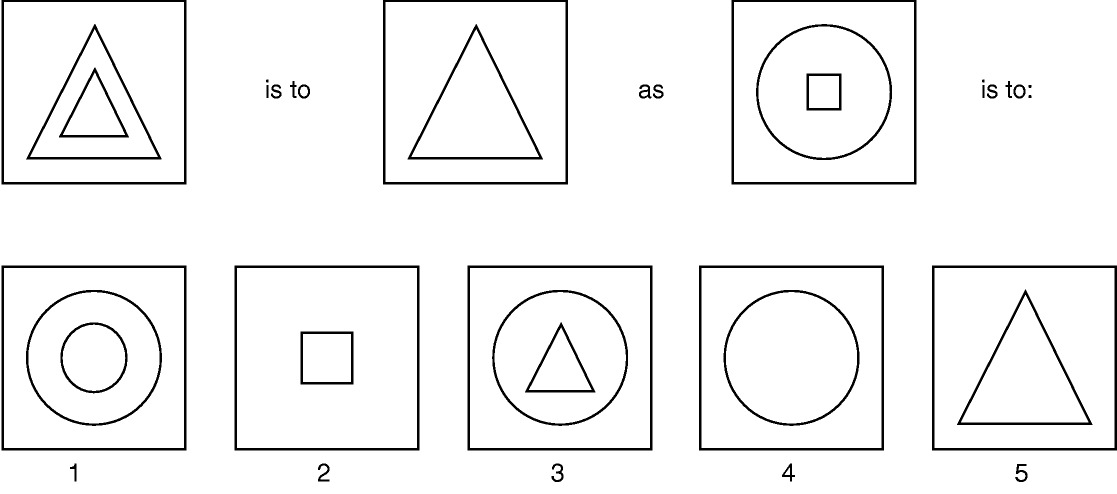
\includegraphics[width=\linewidth]{analogy}
\end{figure}

Um possível algoritmo para resolver esse problema é o seguinte:

\begin{enumerate}
\item Ache uma operação que relaciona os objetos\footnote{Usaremos
    ``objeto'' como um termo geral para nos referir a algo a que não
    queremos nos dar ao trabalho de definir rigorosamente.} para os
  quais conhecemos a relação ``is\_to'';
\item Aplique essa operação no objeto dado para gerar um outro objeto;
\item Cheque se o objeto gerado está entre as opções listadas:
  \begin{itemize}
  \item Se não estiver, volte ao passo (1);
  \item Caso contrário, termine.
  \end{itemize}
\end{enumerate}

No problema específico mostrado, podemos ver que, na primeira linha, a
relação entre o primeiro diagrama e o segundo é que o segundo é o
primeiro quando se retira a figura no centro. Assim, uma resposta ao
problema seria encontrar um diagrama na segunda linha que corresponda
ao terceiro da primeira menos a figura do centro (isto é, um círculo
dentro de um quadrado, o diagrama 4 na segunda linha).

O programa a seguir implementa esses passos em um programa
lógico\footnote{O ``='' usado nesse programa é o mesmo da
``substituição'' mencionada acima e é a relação de identidade: A = B
$\Leftrightarrow$ A é idêntico a B.}:

\begin{listing}
  \inputminted{prolog}{../Exemplos/Cap1/prog3_analogy.pl}
  \caption{Analogy}
\end{listing}

Esse programa é muito específico: ele toma a analogia entre apenas
dois objetos e, a partir disso, cria uma analogia com um terceiro. Uma
generalização é possível, mas, para nossos propósitos, isso é o
suficiente.

Para que ele funcione, a maneira como os diagramas são representados é
fundamental. Estando representados apropriadamente, \funtor{match/3}
nos dá a operação que relaciona um objeto A com um B. Com isso em
mãos, só precisamos aplicar a mesma operação ao termo C, por meio de
\funtor{match/2}, achando X, o objeto que queríamos. Vale ressaltar
que \funtor{match/2} está sendo usado de duas maneiras
diferentes\footnote{Esse tipo de comentário provém de uma leitura
procedural: do ponto de vista estritamente lógico, \funtor{match/2}
apenas expressa uma relação, que pode ser verdadeira ou falsa (isto é,
pode existir ou não existir). Pensar do ponto de vista lógico é
conveniente para fazermos programas mais elegantes e gerais, mas, sem
uma leitura procedural adequada, não conseguiríamos trabalhar com
alguns dos programas que veremos mais para frete.}: para encontrar a
relação entre dois termos e para ``fabricar'' um termo com uma relação
desejada. O predicado \funtor{member/2} ainda não foi explicado, e só
o será melhor entendido posteriormente: por enquanto, é suficiente
assumir que \codigo{member(A, B)} se \var{B} for uma lista (essa coisa
entre colchetes, que será explicada adiante) da qual \var{A} faz parte
(no caso, de C fazer parte de \var{Answers})\footnote{Caso o mistério
te incomode, considere fazer uma visita ao Capítulo 3.}.

Caso esteja se perguntando qual a relação com o modelo do gera-e-testa
discutido anteriormente: o primeiro \technical{match} ajuda o segundo
a gerar o \technical{member} testa se o resultado é válido.

O seguinte programa realiza um teste ao programa anterior:

% \lstinputlisting[caption=TestAnalogy]{../Exemplos/Cap1/prog4_testanalogy.pl}
\begin{listing}
  \inputminted{prolog}{../Exemplos/Cap1/prog4_testanalogy.pl}
  \caption{Test Analogy}
\end{listing}

O goal \codigo{test\_analogy(test1, X)?} tem o resultado esperado.

Talvez tenha estranhado que os últimos programas estejam todos em
inglês. O programa Analogy (um parecido, em espírito, com o usado
aqui) foi apresentado como a tese de doutorado de Thomas Evans
\cite{evans}, no MIT. Preferimos manter o nome original (analogy) e
com o nome veio o resto.

Alguém poderia dizer que a maior parte da ``inteligência'' do programa
está na representação utilizada.  Vale notar, entretanto, que,
diferente do programa discutido aqui, o original não tomava figuras
geométricas como primitivas e tinha que criar um tipo de representação
por conta própria. Como isso foi feito está além do escopo deste
texto.


\begin{thebibliography}{1}

\bibitem{robinson} J.A. Robinson (Jan 1965), ``A Machine-Oriented
  Logic Based on the Resolution Principle'', Journal of the ACM, 12
  (1): 23–41.

\bibitem{evans} T.G. Evans, “A Program for the Solution of
  Geometric-Analogy Intelligence Test Questions”, Semantic Information
  Processing , M. Minsky, ed., MIT Press, 1968, pp. 271–351.

\end{thebibliography}


%\end{document}
